\documentclass[11pt,a4paper]{ctexart}

\usepackage[a4paper,margin=1in]{geometry}
\usepackage[colorlinks=true,linkcolor=blue,urlcolor=blue,citecolor=blue]{hyperref}
\usepackage{booktabs}
\usepackage{tabularx}
\usepackage{array}
\usepackage{enumitem}
\usepackage{float}
\usepackage{xcolor}
\usepackage{graphicx}
\usepackage{tikz}
\usepackage{caption}
\usepackage{amsmath}
\usepackage{amssymb}
\usepackage{multirow}
\usepackage{longtable}
\usetikzlibrary{arrows.meta,positioning}

\definecolor{goodgreen}{rgb}{0.0,0.5,0.0}
\definecolor{todocolor}{rgb}{0.8,0.0,0.0}
\newcommand{\todo}[1]{\textcolor{todocolor}{[\textbf{TODO}: #1]}}
\newcommand{\pending}[1]{\textcolor{todocolor}{#1}}

%% =====================================================================
\title{TransChromBP：基于 Transformer 的碱基分辨率\\
染色质可及性预测模型}

\author{周正伟 \todo{完善作者信息与单位}}
\date{初稿\quad 2026 年 3 月}

%% =====================================================================
\begin{document}
\maketitle

%% =====================================================================
\begin{abstract}
%% =====================================================================

染色质可及性测序（ATAC-seq）是研究基因组调控元件的核心技术。在碱基分辨率层面
对 ATAC-seq 信号进行建模，要求模型同时准确预测插入信号的空间分布（profile）
和总读段计数（count），这对理解转录因子结合位点的精细结构具有重要意义。
ChromBPNet 通过偏差因子化（bias factorization）机制将实验酶切偏好与真实调控信号
分离，为这一任务建立了有效的方法学框架。然而，其卷积主干的感受野有限，难以
捕捉远距离的序列调控依赖关系。

本文提出 TransChromBP 模型，将局部卷积编码、Transformer 自注意力和 ChromBPNet
风格的偏差因子化统一到同一框架中，用于碱基分辨率 ATAC-seq profile/count 预测。
除了报告最终融合输出（full）指标外，本文还显式报告仅由信号分支产生的
debiased 指标，并以 full/debiased gap 作为 bias reliance 的诊断口径。受控复核表明，
在显式 debiased profile supervision 存在时，无论 Transformer scaffold 还是
conv-only scaffold，full/debiased gap 都保持较低；相较之下，去除 debiased profile
supervision 会带来可见但仍属轻度的 bias reliance 增强。这说明 debiased supervision
是当前框架中更关键的稳定因素，而 stop-gradient 更适合作为辅助性的 bias-isolation
设计来理解。

在 ENCODE K562 tutorial benchmark 上，TransChromBP 的主 scaffold 在三个随机种子上
达到 $0.3142 \pm 0.0001$ 的 peak profile JSD 和 $0.8368 \pm 0.0053$ 的 peak count
相关系数；最终 center-pool 默认模型在两个 held-out 种子上进一步达到
$0.3146 \pm 0.0001$ 的 peak profile JSD 和 $0.8496 \pm 0.0010$ 的 peak count
相关系数，并在 clean shortcut test 中保持 $0.00268$ 的低 full/debiased gap。在
matched 的 tutorial \texttt{L3} shared-region system compare 上，TransChromBP 相对
official ChromBPNet 进一步达到更优的 peak mean/median JSD
（$0.31319/0.31547$ vs $0.33853/0.33989$）和更高的 peak count 相关系数
（$0.84016$ vs $0.69958$），说明优势在共享 peaks/nonpeaks/bigWig 的外部对比下
仍然成立。
此外，模型在独立 GM12878 和独立 K562 数据上也获得了稳定的 held-out 结果。
本文还探索了 Genos-1.2B 的融合方案，但未观察到正向收益，提示冻结的全局
foundation-model summary 与碱基分辨率任务之间存在明显的粒度不匹配。

\bigskip
\noindent\textbf{关键词：}
ATAC-seq\quad 碱基分辨率建模\quad Transformer\quad 偏差因子化\quad
Bias reliance 诊断\quad 染色质可及性

\end{abstract}

\tableofcontents
\newpage

%% =====================================================================
\section{引言}
\label{sec:intro}
%% =====================================================================

%% -------------------------------------------------------------------
\subsection{研究背景}
\label{sec:intro-bg}
%% -------------------------------------------------------------------

染色质可及性是真核基因组调控的基本特征。在开放染色质区域（open chromatin regions），
DNA 脱离核小体包裹而暴露出来，使转录因子能够结合到调控元件上，驱动基因表达\cite{buenrostro2013transposition}。
ATAC-seq（Assay for Transposase-Accessible Chromatin using sequencing）利用
Tn5 转座酶优先在开放区域插入测序接头的特性，能够以少量细胞高效地绘制全基因组
染色质可及性图谱，已成为表观基因组学研究中应用最广泛的实验技术之一。

从 ATAC-seq 数据中提取调控信息，可以在不同的分辨率层面进行。传统的峰检测方法
（如 MACS2）在区域级别识别开放染色质位点；而碱基分辨率的信号建模则进一步要求
在每个基因组窗口内预测 Tn5 插入信号的精确空间分布（profile）和总读段计数（count）。
后者对于理解转录因子结合足迹（footprint）的精细结构、区分相邻的调控元件、
以及揭示顺式调控语法（cis-regulatory syntax）具有不可替代的价值。

%% -------------------------------------------------------------------
\subsection{相关工作}
\label{sec:related}
%% -------------------------------------------------------------------

\subsubsection{碱基分辨率信号预测}

BPNet\cite{avsec2021base} 首次提出了碱基分辨率 profile 预测的方法学框架。
该模型使用膨胀卷积（dilated convolution）网络编码 DNA 序列，采用
多项式负对数似然（multinomial NLL）作为 profile 损失函数，用均方误差回归
总 count 的对数值。这一框架建立了 profile + count 双头预测的基本范式，
至今仍是该领域的标准。

ChromBPNet\cite{pampari2023chrombpnet} 在 BPNet 基础上引入了偏差因子化
（bias factorization）机制。其核心思想是：ATAC-seq 信号中混杂了 Tn5 转座酶的
序列切割偏好，这种酶切偏差（enzymatic bias）与真实的转录因子结合信号是
可分离的。ChromBPNet 首先在非峰区域（non-peak regions，其信号主要来源于酶切偏好）
训练一个独立的偏差模型，然后在主训练阶段冻结偏差模型核心参数，让主模型学习
预测去偏后的调控信号。最终预测是信号分支和偏差分支输出的加和。这种因子化设计
显著提升了转录因子 motif 发现和足迹分析的可靠性。

\subsubsection{Transformer 在基因组学中的应用}

自注意力机制能够建模序列中任意位置之间的依赖关系，因此 Transformer 架构
在基因组序列建模中受到广泛关注。Enformer\cite{avsec2021effective} 首次将
Transformer 应用于基因表达预测，使用 196\,kb 的输入窗口捕捉远距离增强子-启动子
相互作用，显著优于纯卷积的 Basenji 模型。DNABERT\cite{ji2021dnabert} 和
Nucleotide Transformer\cite{dallachiesa2023nucleotide} 采用预训练-微调的范式，
在大规模基因组数据上自监督预训练，再迁移到下游任务。

AlphaGenome 将 Transformer 与知识蒸馏（distillation）结合，在更长的上下文窗口上
实现了多任务基因组预测。Genos\cite{genos2025} 提出了参数量达 1.2B--10B 的
基因组基础模型，在多种基因组基准任务上展示了预训练表征的迁移能力。

然而，上述 Transformer 模型大多面向序列级别的分类或回归任务，尚未系统探索
Transformer 在碱基分辨率 ATAC-seq profile 预测中的应用，特别是与偏差因子化机制
的交互效应。

%% -------------------------------------------------------------------
\subsection{研究动机与核心问题}
\label{sec:motivation}
%% -------------------------------------------------------------------

ChromBPNet 的卷积主干感受野约为数百碱基对，这限制了模型捕捉远距离调控依赖的能力。
一个自然的想法是用 Transformer 替换或增强卷积主干，以利用自注意力机制的
长程建模优势。

然而，仅把 Transformer 与偏差因子化直接叠加，并不能保证模型真正学到了去偏后的
调控信号。我们在早期探索中观察到：某些配置虽然 full profile 指标看起来合理，
但 debiased 指标会明显更差，提示模型可能对偏差分支产生依赖。为了避免把探索阶段
的现象直接写成机制定论，本文不把“shortcut 是否存在”预设为结论，而是把
\texttt{full/debiased} 双口径诊断纳入方法与实验主线，用受控对照区分真实表征提升与
bias reliance。

因此，本文真正要回答的核心问题是：
\begin{enumerate}[leftmargin=2em]
  \item 如何在 bias-factorized base-resolution ATAC 建模中安全地接入 Transformer；
  \item 如何诊断模型是否过度依赖偏差分支，而不是只看 full output；
  \item 在满足 bias-safe 条件下，哪些结构设计能够稳定带来主指标收益。
\end{enumerate}

%% -------------------------------------------------------------------
\subsection{本文贡献}
\label{sec:contributions}
%% -------------------------------------------------------------------

本文的主要贡献包括：

\begin{enumerate}[leftmargin=2em]
  \item \textbf{提出 TransChromBP 模型}。将卷积局部编码、Transformer 自注意力
  主干和 ChromBPNet 风格的偏差因子化融合为统一架构，在碱基分辨率 ATAC-seq
  预测任务上显著优于 ChromBPNet 基线。

  \item \textbf{提出 bias reliance 的双口径诊断框架}。同时报告 full 与 debiased
  指标，并以 full/debiased gap 作为定量诊断手段，用于识别模型是否过度依赖
  偏差分支。

  \item \textbf{通过受控复核厘清稳定因素}。clean matrix 结果表明，
  \texttt{debiased profile supervision} 是当前框架中更关键的稳定因素；相比之下，
  stop-gradient 更适合作为辅助性的 bias-isolation 设计来理解。

  \item \textbf{系统验证结构收益与最终默认模型}。通过 Transformer 消融、
  clean shortcut probe 和读出头对比，证明 Transformer 的收益来自真实表征提升，
  并将 \texttt{center pool} 收敛为当前最稳的默认读出头配置。

  \item \textbf{基础模型融合的负结果分析}。探索了 Genos-1.2B 基因组基础模型的
  多种融合策略，得到了有价值的负结论，为基础模型在碱基分辨率任务上的应用
  提供了经验参考。
\end{enumerate}

%% =====================================================================
\section{方法}
\label{sec:method}
%% =====================================================================

%% -------------------------------------------------------------------
\subsection{任务定义}
\label{sec:task}
%% -------------------------------------------------------------------

给定一段长度为 $L = 2114$\,bp 的 DNA 序列，模型需要同时预测中心 1000\,bp 窗口
内的两个目标：

\begin{itemize}[leftmargin=2em]
  \item \textbf{Profile 预测}。在 1000 个碱基位置上预测 Tn5 插入信号的空间分布。
  形式化为多项式分布的参数估计：模型输出 1000 维 logits 向量，经 softmax 后
  表示各位置的插入概率。
  \item \textbf{Count 预测}。预测该窗口内 Tn5 插入的总计数（取对数后为连续标量）。
\end{itemize}

训练数据包含两类区域：峰区域（peaks，以信号峰 summit 为中心）和非峰区域
（nonpeaks，GC 含量匹配的负对照区域）。偏差模型仅在非峰区域上预训练，
主模型在两类区域上联合训练。

%% -------------------------------------------------------------------
\subsection{模型架构}
\label{sec:arch}
%% -------------------------------------------------------------------

TransChromBP 的整体架构如图~\ref{fig:arch} 所示，包含信号分支
（signal branch）、偏差分支（bias branch）和融合模块三部分。

\begin{figure}[H]
\centering
\resizebox{\textwidth}{!}{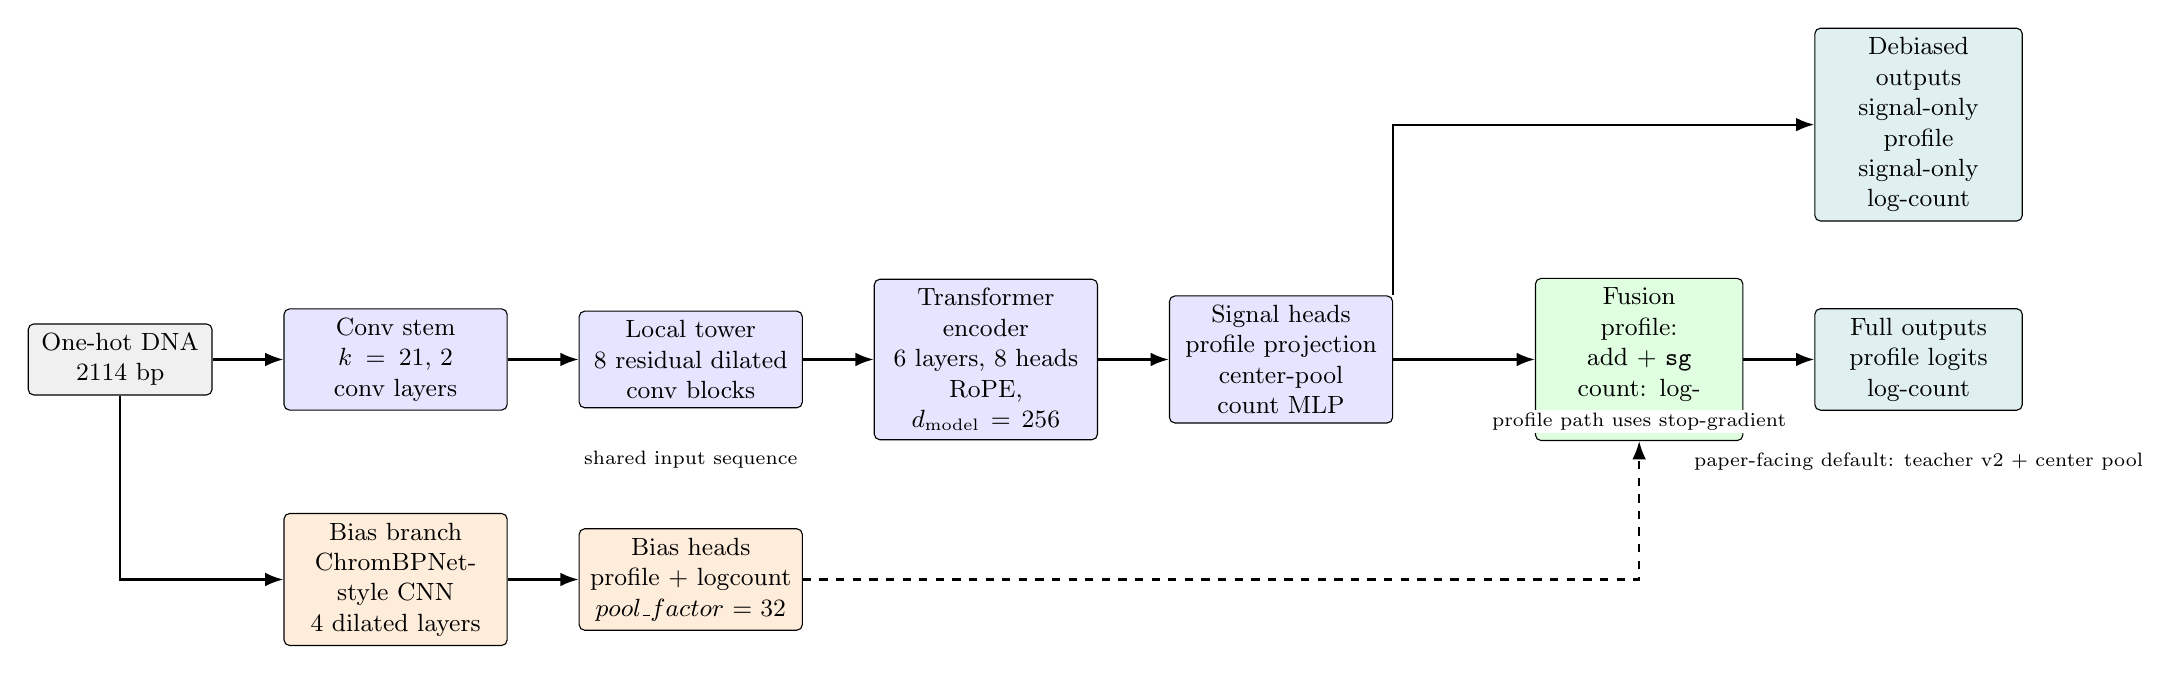
\begin{tikzpicture}[
  font=\small,
  >=Latex,
  node distance=7mm and 9mm,
  data/.style={draw, rounded corners=2pt, align=center, minimum height=9mm, text width=21mm, fill=gray!12},
  sig/.style={draw, rounded corners=2pt, align=center, minimum height=9mm, text width=26mm, fill=blue!10},
  bias/.style={draw, rounded corners=2pt, align=center, minimum height=9mm, text width=26mm, fill=orange!14},
  fuse/.style={draw, rounded corners=2pt, align=center, minimum height=9mm, text width=24mm, fill=green!12},
  outbox/.style={draw, rounded corners=2pt, align=center, minimum height=9mm, text width=24mm, fill=teal!12},
  arrow/.style={-Latex, thick},
  sg/.style={-Latex, thick, dashed},
  note/.style={font=\scriptsize, inner sep=1pt, fill=white}
]

\node[data] (dna) {One-hot DNA\\2114 bp};

\node[sig, right=of dna] (stem) {Conv stem\\$k=21$, 2 conv layers};
\node[sig, right=of stem] (tower) {Local tower\\8 residual dilated\\conv blocks};
\node[sig, right=of tower] (tf) {Transformer encoder\\6 layers, 8 heads\\RoPE, $d_{\text{model}}=256$};
\node[sig, right=of tf] (signal) {Signal heads\\profile projection\\center-pool count MLP};

\node[bias, below=13mm of stem] (biasnet) {Bias branch\\ChromBPNet-style CNN\\4 dilated layers};
\node[bias, right=of biasnet] (biasheads) {Bias heads\\profile + logcount\\$pool\_factor=32$};

\node[fuse, right=18mm of signal] (fusion) {Fusion\\profile: add + \texttt{sg}\\count: log-sum-exp};
\node[outbox, right=of fusion] (full) {Full outputs\\profile logits\\log-count};
\node[outbox, above=11mm of full] (deb) {Debiased outputs\\signal-only profile\\signal-only log-count};

\draw[arrow] (dna) -- (stem);
\draw[arrow] (stem) -- (tower);
\draw[arrow] (tower) -- (tf);
\draw[arrow] (tf) -- (signal);

\draw[arrow] (dna.south) |- (biasnet.west);
\draw[arrow] (biasnet) -- (biasheads);

\draw[arrow] (signal) -- (fusion);
\draw[sg] (biasheads.east) -| (fusion.south);
\node[note, above=1mm of fusion.south] {profile path uses stop-gradient};

\draw[arrow] (fusion) -- (full);
\draw[arrow] (signal.north east) |- (deb.west);

\node[note, below=5mm of tower] {shared input sequence};
\node[note, below=5mm of full] {paper-facing default: teacher v2 + center pool};

\end{tikzpicture}
}
\caption{TransChromBP 的 paper-facing 默认架构。上路是 \texttt{Conv stem + local tower + Transformer}
构成的 signal branch，下路是 ChromBPNet-style bias branch；profile 路径在融合时对
bias profile 使用 stop-gradient，而 count 路径在 log space 中做 log-sum-exp 融合。}
\label{fig:arch}
\end{figure}

\subsubsection{信号分支}

信号分支负责从 DNA 序列中提取去偏后的调控信号，由以下三个模块串联组成：

\paragraph{卷积编码层。}
输入的 one-hot 编码序列 $\mathbf{x} \in \{0,1\}^{L \times 4}$ 首先通过一个一维
卷积 stem（卷积核大小 21，输出维度 $d_{\text{model}}=256$），接 GELU 激活和
Dropout（0.1），提取碱基级别的局部特征。随后经过一个由残差膨胀卷积块组成的
局部塔（local tower），膨胀率按 $2^0, 2^1, \ldots, 2^7$ 指数递增，共 8 层，
用于捕捉 motif 级别的局部序列模式和近邻组合关系；stem 之后还保留两层
卷积核大小为 7 的卷积层作为局部混合。

\paragraph{Transformer 编码器。}
局部塔的输出被送入 Transformer 编码器，由 6 层自注意力模块组成。每层包含
8 头多头自注意力（采用旋转位置编码 RoPE 注入位置信息）、GELU 门控前馈网络和
Pre-Norm 残差连接；前馈维度 $d_{\text{ff}}=4d_{\text{model}}=1024$，Dropout
同样固定为 0.1。Transformer 使序列中任意两个位置都能直接交互，从而建模超出
卷积感受野的远距离调控依赖。

\paragraph{预测头。}
Transformer 的输出通过两个独立的预测头映射为最终预测：

\begin{itemize}[leftmargin=2em]
  \item \textbf{Profile 头}：逐位置的线性投影（$d_{\text{model}} \to 1$），
  随后中心裁剪到 1000\,bp，输出 profile logits。
  \item \textbf{Count 头}：对 Transformer 输出在中心 1000\,bp 范围内进行均值池化
  （center pool），再通过两层 MLP（LayerNorm → Linear → GELU → Dropout → Linear）
  映射为标量 log-count。中心池化确保池化窗口与监督目标的空间范围一致，
  避免两端上下文区域稀释 count 信号。
\end{itemize}

\subsubsection{偏差分支}

偏差分支是一个独立的小型卷积网络，架构与 ChromBPNet 的偏差模型相同：
卷积 stem + 膨胀卷积塔 + profile 头 + count 头。
该分支在非峰区域上预训练，学习预测由 Tn5 酶切偏好主导的背景信号模式。
预训练完成后，偏差分支的核心参数被冻结，仅保留可学习的尺度参数
$\alpha_p$（profile）和 $\alpha_c$（count），用于调节偏差分支对最终预测的贡献强度。
两个尺度参数初始化为 1.0，通过 softplus 函数约束为正值。

\subsubsection{融合模块与 Bias-Safe 设计}

信号分支和偏差分支的输出通过以下方式融合为最终预测：

\begin{align}
  \text{profile}_{\text{full}} &= \text{profile}_{\text{signal}}
    + \alpha_p \cdot \texttt{sg}(\text{profile}_{\text{bias}})
    \label{eq:fusion-profile} \\
  \text{logcount}_{\text{full}} &= \log\bigl(
    \exp(\text{logcount}_{\text{signal}})
    + \alpha_c \cdot \exp(\text{logcount}_{\text{bias}})
  \bigr)
    \label{eq:fusion-count}
\end{align}

其中 $\texttt{sg}(\cdot)$ 表示 stop-gradient 操作。本文将它作为一种
bias-isolation 设计：在 profile 融合路径上截断梯度，使得 profile 损失
不会通过偏差分支的 profile 输出回传。这样可以更好地维持 signal branch 与
bias branch 的功能分工，并降低模型在训练中对偏差分支产生额外依赖的风险。

值得注意的是，count 融合路径（公式~\ref{eq:fusion-count}）\textbf{不}施加
stop-gradient，因为偏差分支对 count 的贡献是合理的——酶切偏好确实会影响
区域的整体可及性读数。Profile 和 count 路径上偏差分支角色的不对称性，是本文
融合设计的核心考量。

%% -------------------------------------------------------------------
\subsection{训练策略}
\label{sec:training}
%% -------------------------------------------------------------------

训练分为两个阶段：

\paragraph{阶段一：偏差预训练。}
仅训练偏差分支，数据源为非峰区域。偏差分支学习预测酶切偏好主导的背景信号。

\paragraph{阶段二：主模型训练。}
冻结偏差分支核心参数，训练信号分支（含 Transformer）和尺度参数。
数据包含峰区域和非峰区域。

训练损失函数为：
\begin{equation}
  \mathcal{L} = \mathcal{L}_{\text{profile}}^{\text{full}}
    + \lambda_c \cdot \mathcal{L}_{\text{count}}^{\text{full}}
    + \lambda_d \cdot \mathcal{L}_{\text{profile}}^{\text{debiased}}
  \label{eq:loss}
\end{equation}
其中 $\mathcal{L}_{\text{profile}}$ 为多项式负对数似然，
$\mathcal{L}_{\text{count}}$ 为对数 count 的均方误差，
$\lambda_c$ 为 count 损失权重（自动标定），
$\lambda_d$ 为 debiased profile 损失权重。
Debiased 损失项鼓励信号分支独立产生高质量的 profile 预测。

优化器使用 AdamW（学习率 $5\times 10^{-4}$、$\beta=(0.9,0.95)$、
权重衰减 $0.01$），学习率调度采用 cosine annealing 并带线性 warmup，
warmup 比例为 0.06，最小学习率比例为 0.1。训练过程中使用 bf16 混合精度。
数据增强包括 $\pm 500$\,bp 的随机平移（jitter）和反向互补
（reverse complement，概率 0.5）。tutorial backbone 与 clean-matrix 系列
通常训练 30 个 epoch；readout-head 收口使用 40 个 epoch；shared-region
strict-compare 使用 50 个 epoch。双卡 run 默认 \texttt{batch\_size\_per\_gpu=16}
（effective batch 为 32）；6000 单卡确认 run 则通过 \texttt{grad\_accum=2} 保持相同
有效 batch 量级。

%% -------------------------------------------------------------------
\subsection{评估指标}
\label{sec:metrics}
%% -------------------------------------------------------------------

模型评估使用以下指标，均在 held-out 测试集（染色体 1）上计算：

\begin{itemize}[leftmargin=2em]
  \item \textbf{Peak profile JSD}。每个峰区域上预测分布与观测分布的
  Jensen-Shannon 散度，在所有峰区域上取均值。越低越好。
  \item \textbf{Peak count $r$}。所有峰区域上预测 count 与观测 count 的
  Pearson 相关系数。越高越好。
  \item \textbf{Debiased profile JSD}。仅使用信号分支输出（不含偏差分支贡献）
  计算的 profile JSD。用于诊断 bias reliance。
  \item \textbf{Full/debiased 差距}。Full JSD 与 debiased JSD 之差。
  差距越大，说明模型对偏差分支的依赖越强。
\end{itemize}

%% =====================================================================
\section{实验}
\label{sec:experiments}
%% =====================================================================

%% -------------------------------------------------------------------
\subsection{实验设置}
\label{sec:setup}
%% -------------------------------------------------------------------

\subsubsection{数据集}

主要实验使用 ENCODE K562 ATAC-seq 数据集（ChromBPNet 官方教程数据），
包含三个生物学重复的合并 BAM 文件。峰位点以 summit 为中心提取，非峰区域为
GC 含量匹配的负对照。染色体划分遵循 ChromBPNet 标准 fold 配置，
染色体~1 保留为 held-out 测试集。信号使用无链偏移的 Tn5 插入 bigWig 文件。

跨数据集验证使用两套独立的 ENCODE ATAC-seq 数据集：GM12878 和 K562
（与教程数据使用不同的 replicate 配置和预处理流程），经相同的预处理管线产生
独立的峰集合、非峰对照和 bigWig 信号。

\subsubsection{对比方法}

\begin{itemize}[leftmargin=2em]
  \item \textbf{ChromBPNet}：官方教程配置的复现结果，使用纯卷积主干和偏差因子化。
  本文同时保留两种外部比较口径：历史 tutorial baseline，以及 matched 的
  \texttt{L3} shared-region controlled arm。
  \item \textbf{TransChromBP（无 Transformer）}：去除 Transformer 模块的变体，
  仅保留卷积主干和偏差因子化，用于隔离 Transformer 的独立贡献。
  \item \textbf{Bias reliance clean matrix}：包括 \texttt{TF + sg=false + deb2}、
  \texttt{TF + sg=true + deb0}、\texttt{noTF + sg=false + deb2} 与
  \texttt{noTF + sg=true + deb0} 四个格子的 \texttt{split=test} 结果；此外再报告
  paper-facing 的 \texttt{corrected B} test，用于区分“机制诊断 scaffold”与
  “最终默认模型”的安全性。
\end{itemize}

\subsubsection{实验配置}

主 benchmark、Transformer/backbone 消融以及大部分 tutorial 主线训练在
NVIDIA A6000（$2 \times 48$\,GB 显存）上完成；独立真实数据验证、部分
shortcut 复核和若干 confirmatory run 在单卡 RTX 3080 上完成。除特殊说明外，
正文中所有表格都会显式标注 seed 数：主 backbone 消融使用三个随机种子
（42, 1234, 2024）；\texttt{TF + sg=true + deb0} 这条 unsafe TF 条件当前
已经补齐两个 test seed；而最终 \texttt{center pool} 默认模型当前使用两个
held-out seed 作为 readout 收口依据。

%% -------------------------------------------------------------------
\subsection{主要结果}
\label{sec:main-result}
%% -------------------------------------------------------------------

表~\ref{tab:main} 采用“双轨并列”的方式组织外部比较。上半部分保留历史
tutorial baseline，用来和公开可复用的外部数字建立延续关系；下半部分则给出
本轮已经收口的 \texttt{L3} shared-region system compare，用 matched 的
peaks/nonpeaks/bigWig 提供更强的受控比较。两部分回答的是不同层次的问题，
因此不应混成单一数值排序。

\begin{table}[H]
\centering
\small
\caption{TransChromBP 与 ChromBPNet 的双轨外部比较。Panel A 保留历史 tutorial
参考；Panel B 给出 matched 的 \texttt{L3} shared-region system compare。}
\label{tab:main}
\textbf{Panel A. 历史 tutorial 参考}\\[2mm]
\resizebox{\textwidth}{!}{%
\begin{tabular}{lcccc}
\toprule
模型 & Peak profile JSD $\downarrow$ & 聚合方式 & Peak count $r$ $\uparrow$ & 说明 \\
\midrule
ChromBPNet（官方 tutorial） & $0.3360$ & median & $0.7274$ & 历史外部参考 \\
TransChromBP corrected B（2 seeds） & $\mathbf{0.3146 \pm 0.0001}$ & mean & $\mathbf{0.8496 \pm 0.0010}$ & 当前默认 readout \\
\bottomrule
\end{tabular}
}

\vspace{2mm}
\textbf{Panel B. \texttt{L3} shared-region system compare}\\[2mm]
\resizebox{\textwidth}{!}{%
\begin{tabular}{lcccc}
\toprule
模型 & Peak mean JSD $\downarrow$ & Peak median JSD $\downarrow$ & Peak count $r$ $\uparrow$ & 说明 \\
\midrule
Official ChromBPNet controlled L3 & $0.33853$ & $0.33989$ & $0.69958$ & matched peaks/nonpeaks/bigWig \\
TransChromBP corrected-B controlled L3 & $\mathbf{0.31319}$ & $\mathbf{0.31547}$ & $\mathbf{0.84016}$ & 同一 shared-region 设置 \\
\bottomrule
\end{tabular}
}
\end{table}

Panel A 主要说明：即便沿用历史 tutorial baseline，TransChromBP 的默认
\texttt{corrected B} readout 在 count 分支上也仍然明显优于公开的
ChromBPNet baseline（$0.8496$ vs $0.7274$）；而 profile 列由于 median/mean
口径不同，更适合作为“竞争力和改善趋势”的外部参考。Panel B 则提供当前更强的
受控证据：在完全共享 peaks/nonpeaks/bigWig 的 \texttt{L3} 设定下，TransChromBP
在 peak mean JSD、median JSD 与 count\_r 三项上都优于 official，
对应改善分别为 $0.02534$、$0.02442$ 和 $0.14058$。因此，本文的外部比较主结论
应建立在“历史 tutorial 参考 + matched shared-region compare”这两条证据的组合上，
而不是继续只依赖旧的单轨 baseline 表。

\subsubsection{L3 shared-region 的分类附表}

作为 supplementary 风格的辅助比较，我们还在 \texttt{L3} shared-region 上报告
peak-vs-nonpeak 分类指标（表~\ref{tab:l3-classification}）。这组指标不进入主表，
但和 profile/count 的方向一致：TransChromBP 在 AUROC/AUPRC/F1 三项上都优于
official。由于 official 侧的分类字段是通过同一条 held-out test 链路补齐的，
这里把它作为附表证据，而不是单独扩成新的主叙事。

\begin{table}[H]
\centering
\small
\caption{\texttt{L3} shared-region 的 supplementary 风格分类附表。}
\label{tab:l3-classification}
\begin{tabular}{lccc}
\toprule
模型 & AUROC $\uparrow$ & AUPRC $\uparrow$ & Best F1 $\uparrow$ \\
\midrule
Official ChromBPNet controlled L3 & $0.82295$ & $0.83148$ & $0.75248$ \\
TransChromBP corrected-B controlled L3 & $\mathbf{0.87861}$ & $\mathbf{0.87530}$ & $\mathbf{0.80991}$ \\
\bottomrule
\end{tabular}
\end{table}

%% -------------------------------------------------------------------
\subsection{Bias Reliance 诊断与受控复核}
\label{sec:shortcut-analysis}
%% -------------------------------------------------------------------

\subsubsection{为什么需要 Full/Debiased 双口径}

在 bias factorization 架构中，仅报告最终融合输出（full）并不足以判断信号分支
是否真正学到了去偏后的调控模式。为此，本文同时报告：

\begin{itemize}[leftmargin=2em]
  \item \textbf{full 指标}：使用最终融合输出计算的 profile/count 指标；
  \item \textbf{debiased 指标}：仅使用 signal branch 输出计算的指标；
  \item \textbf{full/debiased gap}：用来衡量模型是否对 bias branch 产生额外依赖。
\end{itemize}

早期探索实验曾提示某些配置下 full 与 debiased 差距较大，但这些 run 同时混入了
多个结构和训练目标变化，不能直接作为论文主结论。因此，下面的判断只基于本轮
clean matrix 的 \texttt{split=test} 结果。

\subsubsection{Clean Matrix 结果}

\begin{table}[H]
\centering
\small
\caption{Bias reliance 的 clean revalidation。按本轮预先约定的判读门槛，
A、\texttt{noTF + sg=false + deb2} 和 corrected B 都落在“无实质 shortcut”
区间；C 在两个 seed 上表现为轻度且稳定的 bias reliance，而
\texttt{noTF + sg=true + deb0} 是当前矩阵中唯一达到“明显 shortcut”门槛的
条件。除 C 外，其余各行为单次 held-out test。}
\label{tab:shortcut}
\resizebox{\textwidth}{!}{%
\begin{tabular}{lccccc}
\toprule
Run & 条件 & Peak JSD (full) & Peak JSD (deb) & Full/deb gap & Peak count $r$ (full/deb) \\
\midrule
A & \texttt{TF + sg=false + deb2} & $0.31410$ & $0.31416$ & $0.00147$ & $0.8506 / 0.8488$ \\
C（2 seeds） & \texttt{TF + sg=true + deb0} & $0.31730 \pm 0.00014$ & $0.31787 \pm 0.00011$ & $0.00984 \pm 0.00018$ & $0.8367 \pm 0.0039 / 0.8348 \pm 0.0031$ \\
noTF-safe & \texttt{noTF + sg=false + deb2} & $0.43531$ & $0.43557$ & $0.00487$ & $0.7959 / 0.7966$ \\
noTF-unsafe & \texttt{noTF + sg=true + deb0} & $0.43659$ & $0.43835$ & $0.02682$ & $0.7919 / 0.7956$ \\
corrected B & \texttt{TF + center + sg=true + deb2} & $0.42544$ & $0.42556$ & $0.00268$ & $0.8439 / 0.8420$ \\
\bottomrule
\end{tabular}
}
\end{table}

\subsubsection{受控复核的结论}

当前矩阵与 paper-facing 最终模型给出的结论，与早期 draft 中的强叙事并不一致。

第一，本文没有复现出“Transformer 特有的强 shortcut”。按本轮的
判读门槛，A、noTF-safe 和 corrected B 的 full/debiased gap 都处于“无实质
shortcut”区间；C 在两个 seed 上虽然都出现了 gap 抬升，但量级仍属于
\textbf{轻度且稳定的 bias reliance}；相反，真正达到“明显 shortcut”门槛的
是 conv-only 的 \texttt{noTF + sg=true + deb0}，其 gap 达到 $0.02682$。

第二，当前证据更支持 \texttt{debiased profile supervision} 比 \texttt{stop-gradient}
更关键。A（关掉 \texttt{sg}、保留 \texttt{deb2}）仍然非常干净，而 C（保留
\texttt{sg}、去掉 \texttt{deb2}）在两个 seed 上都出现了可见 gap，这说明在当前
框架中，\texttt{deb2} 更像主效应，\texttt{stop-gradient} 更适合被理解为
辅助性的 bias-isolation 设计。

第三，当前证据已经直接反对 “Transformer 特有” 或 “纯卷积不会出现” 这类架构级
强断言。在显式 debiased supervision 存在时，Transformer scaffold 和 conv-only
scaffold 都可以维持较低的 full/debiased gap；而在同样的 unsafe 配置
（\texttt{sg=true + deb0}）下，conv-only 的 gap 反而高于 TF。这说明当前矩阵更自然
支持“bias reliance 主要由 supervision 是否安全主导”，而不是“由 backbone 是否是
Transformer 主导”。

第四，paper-facing 的最终模型 \texttt{corrected B} 也没有出现明显 shortcut，这一点对于
论文叙事非常关键：最终主模型不是建立在 bias reliance 上“换指标”，而是在保持低
full/debiased gap 的前提下获得了更强的 count 预测。

%% -------------------------------------------------------------------
\subsection{组件消融实验}
\label{sec:component-ablation}
%% -------------------------------------------------------------------

\subsubsection{Transformer 主干的贡献}

为隔离 Transformer 的独立贡献，本文将完整模型（V2-full）与去除 Transformer 模块
的变体（V2-noTF）进行了匹配对照。两组各使用三个随机种子，训练 30 个 epoch，
除 Transformer 模块外其他配置完全相同。

\begin{table}[H]
\centering
\caption{Transformer 消融实验。V2-full 在三个种子上一致优于 V2-noTF，
且 full/debiased 差距保持极小，说明 Transformer 的收益来自真实的表征能力
而非偏差泄露。}
\label{tab:tf-ablation}
\begin{tabular}{lcccc}
\toprule
变体 & Peak JSD $\downarrow$ & Peak count $r$ $\uparrow$
  & Full/deb 差距 & 种子数 \\
\midrule
V2-full（含 TF）
  & $\mathbf{0.31419 \pm 0.00012}$ & $\mathbf{0.83676 \pm 0.00531}$
  & $0.00006$ & 3 \\
V2-noTF（无 TF）
  & $0.32393 \pm 0.00021$ & $0.82503 \pm 0.00489$
  & $0.00010$ & 3 \\
\midrule
差异 & $-0.00974$ ($-3.0\%$) & $+0.01173$ ($+1.4\%$) & & \\
\bottomrule
\end{tabular}
\end{table}

V2-full 在 profile JSD 上改善约 3.0\%（0.010），在 count 相关系数上提升约 1.4\%
（0.012）。全部六组对比（3 种子 $\times$ 2 指标）均支持 V2-full，
符号检验 $p \approx 0.016$。更重要的是，full/debiased 差距保持在 0.00006 的极低
水平，确认 Transformer 的收益不是来自重新引入偏差泄露。

\subsubsection{偏差分支的必要性}

本文当前主结论并不建立在“完全去掉 bias branch”的极端组件消融上。更关键的
证据来自 clean matrix 与 \texttt{L3} shared-region 对比：前者回答模型是否
bias-safe，后者回答 system-level 外部比较是否成立。\texttt{bias\_branch.enabled=false}
的 no-bias 消融因此被定位为补充性的 component-necessity 检查，其结果更适合
进入 supplementary，而不是替代 clean matrix 或双轨主表成为新的主证据。

\texttt{2026-03-31} 完成的单 seed no-bias 补证沿用当前 tutorial canonical
paper-facing recipe，并用外部 valid selector 选出 \texttt{epoch 26}。该 checkpoint
在 held-out \texttt{test-full} 上达到 peak mean/median JSD=\texttt{0.31496/0.31715}、
peak count $r$=\texttt{0.84978}，同时 count-scale 的 peak-vs-nonpeak
\texttt{AUROC/AUPRC/best F1=0.88990/0.88418/0.82037}。这些数字与当前 corrected-B /
center-pool 主配置基本同档，没有显示“去掉 bias branch 后性能必然明显下降”
或“反而显著更强”。因此更准确的写法是：在现有 Transformer + center-pool
recipe 下，显式 bias factorization 在单 seed 上没有体现出清晰的额外收益；
但这条边界结果并不替代 clean matrix 对 bias-safe 的诊断，也不替代
\texttt{L3} shared-region 对外部比较的主证据角色。

\subsubsection{读出头设计}

本文评估了四种读出头变体以理解最终映射层对性能的影响
（表~\ref{tab:readout}）。所有变体共享相同的 Transformer 主干和偏差安全训练框架，
仅在 count 池化策略和/或 profile 头结构上有所不同，统一训练 40 个 epoch。

\begin{table}[H]
\centering
\caption{读出头变体的第一轮对比。表内行为种子 42 的 held-out 结果；
后续 \texttt{B/F} 还补充了 matched seed=1234 的 confirmatory run。}
\label{tab:readout}
\begin{tabular}{llccc}
\toprule
变体 & 设计思路 & Peak JSD $\downarrow$ & Peak count $r$ $\uparrow$
  & Best epoch \\
\midrule
A: Freeze fix & 冻结偏差分支 BN 层 & $0.3148$ & $0.8446$ & 40 \\
B: Center pool & 中心对齐 count 池化 & $\mathbf{0.3147}$ & $\mathbf{0.8503}$ & 34 \\
F: Attention pool & 注意力加权 count 池化 & $0.3148$ & $0.8492$ & 40 \\
G: Profile refine & 可学习 profile 精修头 & $0.4260$ & $0.8460$ & 15 \\
\midrule
基线（V2-full） & 全长均值池化 & $0.3143$ & $0.8354$ & 29 \\
\bottomrule
\end{tabular}
\end{table}

A、B、F 三种变体在 seed 42 上都显著提升了 count 相关系数（$+0.009$ 至 $+0.015$），
同时保持了几乎完全相同的 profile JSD（$0.3147$--$0.3148$）。如果只看这一轮，
三者都可以被视为正向 readout 候选。

但后续的 matched seed=1234 confirmatory run 把 B/F 区分开了：\texttt{B\_s1234} 的 held-out
结果为 $0.3145 / 0.8488$，与 \texttt{B\_s42} 的 $0.3147 / 0.8503$ 几乎同档；相对地，
\texttt{F\_s1234} 的 held-out profile JSD 退化到 $0.4269$，虽然 count 仍有 $0.8457$，
但已经不再满足“稳定保持 profile 主指标”的要求。换言之，\texttt{center pool} 不只是
单 seed 领先，而是当前\textbf{唯一在后续 confirmatory seed 上继续保持稳定}的
readout 方案，因此被选为最终默认配置。

G（profile refine）的结果构成了一个反面案例：增加可学习的 profile 精修层
在 count 上表现尚可，但 profile JSD 急剧恶化（0.4260），说明额外参数
过拟合了训练分布的 profile 形状。其极早的 best epoch（15，远低于其他变体的
29--40）进一步支持了这一解释。

%% -------------------------------------------------------------------
\subsection{基因组基础模型融合实验}
\label{sec:genos}
%% -------------------------------------------------------------------

预训练基因组基础模型在序列级别任务上展现了显著的迁移能力，本文因此探索了将
Genos-1.2B 的表征融入 TransChromBP 的可能性。实验涵盖两种范式共五种融合策略。

\subsubsection{在线融合与缓存融合}

\begin{table}[H]
\centering
\caption{Genos-1.2B 融合实验结果。所有变体与匹配基线 G0 对照。
没有任何策略在两个指标上同时实现正向收益。}
\label{tab:genos}
\begin{tabular}{llcc}
\toprule
策略 & 融合方式 & Peak JSD $\downarrow$ & Peak count $r$ $\uparrow$ \\
\midrule
G0（基线） & 不使用 Genos & $0.3163$ & $\mathbf{0.8410}$ \\
\midrule
G1（gate） & 在线，逐位置门控 & $0.3388$ & $0.4689$ \\
G2（mean） & 在线，全局均值广播 & $0.3387$ & $0.6360$ \\
P0（cached baseline） & 缓存，匹配配置 & $0.3179$ & $0.8384$ \\
P2（count-only） & 缓存，注入 count 头 & $\mathbf{0.3174}$ & $0.6037$ \\
\bottomrule
\end{tabular}
\end{table}

五种策略均未产生正向结果。在线融合（G1、G2）在验证集上看似接近基线，
但 held-out 测试上 count 相关系数严重崩塌（G1 低至 0.469），暴露了严重的
泛化失效。缓存融合的匹配基线（P0）虽然稳定，但未超过 G0。
直接向 count 头注入全局 summary 的 P2 获得了最好的 profile JSD，
但造成了 count 的断崖式下滑（$r = 0.60$）。

\subsubsection{诊断性探针分析}

为理解负结果的原因，本文对缓存的 Genos summary 进行了诊断性探针实验：

\begin{itemize}[leftmargin=2em]
  \item Genos \texttt{global\_mean} 对 count 残差（去除模型自身预测后）仅有
  $R^2 = 0.017$ 的解释力，Pearson $r = 0.199$。
  \item \texttt{genos\_only} 对 peak/nonpeak 二分类的 AUC $= 0.700$，
  确认 summary 中确实包含可及性相关信息。
  \item 但 \texttt{concat(encoded, genos)} 的 AUC $= 0.902$，
  \textbf{低于} \texttt{encoded\_only} 的 AUC $= 0.922$。
\end{itemize}

这组探针揭示了一个关键事实：Genos 的全局 summary 确实携带可及性信息，
但这些信息与 TransChromBP 主干已提取的信息存在较强重叠，
直接拼接反而引入了噪声而非互补信号。

\subsubsection{OCR 基准复现}

为排除实现错误的可能性，本文复现了 Genos 官方的开放染色质区域（OCR）
分类基准。在 \texttt{human\_ocr\_ensembl} 数据集上，本地 Genos-1.2B 使用
layer 12 embedding 取得 ROC AUC $= 0.7535$，与官方报告值 $0.7569$ 仅差 0.5\%。
这确认了本地安装和推理链路完全正常，负结果不是由技术故障导致。

\subsubsection{负结果的原因}

综合上述证据，Genos 融合失败的根本原因是\textbf{任务粒度不匹配}：

\begin{enumerate}[leftmargin=2em]
  \item OCR 分类是序列级别的二值分类任务，天然适合全局均值池化的 summary 表征。
  \item ATAC profile/count 预测是碱基分辨率的空间分布回归，需要局部 motif 组合
  和位置结构信息——这些信息在 \texttt{global\_mean} 池化中丢失了。
  \item 当前 TransChromBP 主干已经很强（G0 baseline 达到 $0.3163 / 0.8410$），
  留给外部弱信号的增量空间极小。
\end{enumerate}

这一分析对基因组基础模型在碱基分辨率任务上的应用具有参考价值：仅靠
冻结的序列级 summary 是不够的，更精细的融合策略（如逐位置特征、
交叉注意力或参数微调）可能是必要的。

%% -------------------------------------------------------------------
\subsection{跨数据集泛化验证}
\label{sec:generalization}
%% -------------------------------------------------------------------

为验证 TransChromBP 并非仅在教程数据上过拟合的产物，本文在 GM12878 和 K562
两套独立 ATAC-seq 数据集上进行了训练和评估。

\begin{table}[H]
\centering
\caption{跨数据集泛化结果。两套数据集的 held-out 测试性能均与验证一致甚至更优，
确认模型不存在特定 split 的过拟合。}
\label{tab:generalization}
\begin{tabular}{lcccc}
\toprule
数据集 & Best epoch & Val peak JSD & Test peak JSD & Test peak count $r$ \\
\midrule
GM12878 & 19 & $0.4302$ & $0.4226$ & $0.8040$ \\
K562 & 35 & $0.6281$ & $0.6124$ & $0.8586$ \\
\bottomrule
\end{tabular}
\end{table}

两个数据集上，held-out 测试性能均达到或超过验证性能，表明模型没有出现
split 特异性失真。GM12878 和 K562 上的 peak JSD 绝对值高于教程数据，
这主要反映了不同数据集固有的峰特征差异和信噪比水平，而非模型性能下降。
两套数据上的 count 相关系数都稳定在 0.80--0.86，表明 count 预测在不同
数据集上的一致性优于 profile。

%% =====================================================================
\section{讨论}
\label{sec:discussion}
%% =====================================================================

%% -------------------------------------------------------------------
\subsection{Bias Reliance 诊断的意义与边界}
%% -------------------------------------------------------------------

本工作的主要方法学价值，不在于“已经证明了某个强而普适的 Transformer 特有
shortcut 机制”，而在于给出了一个更稳妥的 bias reliance 诊断框架：在带有
bias factorization 的架构中，单看 full output 容易掩盖模型对偏差分支的依赖，
而 full/debiased gap 则提供了一个低成本、可复用、能直接落到 held-out test 的
诊断口径。

同样重要的是，当前证据也明确了这套叙事的边界。clean revalidation 支持的，
是“显式 debiased profile supervision 对稳定训练很关键”；暂时\textbf{不支持}的，
则是“强 shortcut 已被稳健复现”以及“这是 Transformer 特有现象”。这意味着本文
在讨论架构风险时必须克制：我们可以提出需要警惕 bias reliance，但不能把当前结果
夸写成已完成的普适机制证明。

从实践角度看，这一结论仍然有价值。未来只要模型同时具备：
\begin{enumerate}[leftmargin=2em]
  \item 高容量主干；
  \item 显式的 bias / confounder 分支；
  \item 可学习的融合路径；
\end{enumerate}
就应优先检查 full/debiased 两套指标是否一致，而不是只依赖 full output 的表观性能。
相比“是否存在某个特定 shortcut”，这种诊断原则更容易迁移到其它带偏差分解的
基因组学模型中。

%% -------------------------------------------------------------------
\subsection{基础模型与任务粒度}
%% -------------------------------------------------------------------

Genos-1.2B 融合实验的负结果为基因组学社区提供了一个受控的经验参考。
核心洞察在于基础模型的有效性强烈依赖于预训练表征的粒度与下游任务的匹配度。

对于序列级别的分类任务（如 OCR 检测），全局均值池化的 embedding 已经足够有效，
这也被本文的 OCR 基准复现所验证。但对于碱基分辨率的回归任务（如 ATAC profile
预测），同样的 embedding 丢失了任务所需的空间信息。

此外，当任务专用的 baseline 已经很强时，外部弱信号越过噪声门槛的难度更大。
这构成了一个"基线悖论"：越是需要外部知识补充的弱 baseline 场景，
外部 summary 的边际收益越容易体现；越是已经被任务专用架构充分优化的强
baseline 场景，外部补充越难产生可检测的增量。

%% -------------------------------------------------------------------
\subsection{局限性与未来工作}
%% -------------------------------------------------------------------

本文存在以下局限性：

\begin{enumerate}[leftmargin=2em]
  \item \textbf{基准规模有限}。主要消融基于单一 ENCODE K562 数据集。
  虽然多数据集实验（GM12878, K562）验证了泛化性，但更大规模的跨细胞系、
  跨测序平台评估将进一步增强结论的说服力。

  \item \textbf{未进行知识蒸馏}。当前框架使用直接训练，未探索 teacher-student
  蒸馏范式。一个更长上下文的 teacher 是否能通过蒸馏将长程知识有效迁移到
  当前窗口的 student，是一个值得探索的方向。

  \item \textbf{基础模型融合策略有限}。本文仅测试了冻结全局 summary 的注入。
  更精细的策略（逐位置特征、交叉注意力、LoRA 微调）可能释放基础模型表征中的
  空间信息。

  \item \textbf{输入窗口固定}。TransChromBP 使用与 ChromBPNet 相同的 2114\,bp
  输入窗口。扩展到更长窗口可能放大 Transformer 的比较优势，但需要相应的
  数据预处理和训练基础设施改造。

  \item \textbf{conv-only unsafe 条件的 seed 方差仍可继续量化}。
  当前 clean matrix 已经包含 \texttt{noTF + sg=true + deb0} 这一 matched control，
  并且其 gap 是当前矩阵最高；但论文主文中这条条件目前仍主要依赖单 seed test。
  未来若继续补 multi-seed，可进一步收紧 conv-only 高 gap 的方差估计。

  \item \textbf{外部 baseline 的 profile 聚合口径不完全一致}。
  ChromBPNet 官方 tutorial 公开的是 peak profile median JSD，而本文主线统一报告
  mean JSD。因此当前外部 profile 对比应被理解为保守参考，而非完全同聚合方式下的
  一一对应比较。
\end{enumerate}

%% =====================================================================
\section{结论}
\label{sec:conclusion}
%% =====================================================================

本文提出了 TransChromBP，将 Transformer 自注意力与 bias factorization
结合到碱基分辨率 ATAC-seq profile/count 预测任务中。当前最稳的结论不是
“我们已经证明了一个强且 Transformer 特有的 Profile Shortcut”，而是：
在带偏差分解的架构里，必须同时检查 full 与 debiased 两套指标，才能判断模型
是否真正学到了去偏后的调控信号。

受控复核表明，显式的 debiased profile supervision 是当前框架中更关键的稳定因素；
在其存在时，Transformer scaffold 与 conv-only scaffold 都可以维持较低的
full/debiased gap。与此同时，Transformer 主干在 tutorial benchmark 上带来了
稳定的主指标收益，而 \texttt{center pool} 读出头进一步把模型收敛为当前最稳的默认配置。

因此，本文的核心贡献应被理解为：提出了一个 bias-safe 的 Transformer
ATAC 建模框架、一套可复用的 bias reliance 诊断口径，以及一个经 held-out
结果支撑的最终默认模型。Genos-1.2B 的负结果则进一步提示，冻结的序列级
summary 表征并不能自然迁移到碱基分辨率任务，任务粒度匹配仍然是基础模型
融合中的关键挑战。

%% =====================================================================
%% 参考文献
%% =====================================================================
\begin{thebibliography}{99}

\bibitem{buenrostro2013transposition}
Buenrostro J D, Giresi P G, Zaba L C, et al.
Transposition of native chromatin for fast and sensitive epigenomic profiling
of open chromatin, DNA-binding proteins and nucleosome position[J].
\emph{Nature Methods}, 2013, 10(12): 1213--1218.

\bibitem{avsec2021base}
Avsec \v{Z}, Weilert M, Shrikumar A, et al.
Base-resolution models of transcription-factor binding reveal soft motif
syntax[J]. \emph{Nature Genetics}, 2021, 53(3): 354--366.

\bibitem{pampari2023chrombpnet}
Pampari A, Shcherbina A, Engelbrecht E, et al.
ChromBPNet: bias factorized, base-resolution deep learning models of
chromatin accessibility reveal cis-regulatory sequence syntax[J].
\emph{bioRxiv}, 2023.

\bibitem{avsec2021effective}
Avsec \v{Z}, Agarwal V, Visentin D, et al.
Effective gene expression prediction from sequence by integrating long-range
interactions[J]. \emph{Nature Methods}, 2021, 18(10): 1196--1203.

\bibitem{ji2021dnabert}
Ji Y, Zhou Z, Liu H, et al.
DNABERT: pre-trained Bidirectional Encoder Representations from Transformers
model for DNA-language in genome[J].
\emph{Bioinformatics}, 2021, 37(15): 2112--2120.

\bibitem{dallachiesa2023nucleotide}
Dalla-Torre H, Gonzalez L, Mendoza-Revilla J, et al.
The Nucleotide Transformer: Building and Evaluating Robust Foundation Models
for Human Genomics[J]. \emph{bioRxiv}, 2023.

\bibitem{genos2025}
BGI-HangzhouAI.
Genos: a pretrained genome foundation model for comprehensive genomic
understanding[J]. \emph{GigaScience}, 2025.

\end{thebibliography}

\end{document}
